\section{项目测试}\label{sec:Project_Testing}

\subsection{引言}

单元测试是现代软件开发中至关重要的一环,它帮助确保代码的正确性、可靠性和稳定性。对于PetJoy项目,单元测试不仅能够验证各个组件的功能实现,还能在项目迭代中及时发现和修复潜在问题。特别是前端开发中,单元测试有助于提升用户体验和代码质量。

\subsection{单元测试的重要性}

在PetJoy项目中,单元测试具有以下几方面的重要性:

\begin{itemize}
    \item \textbf{确保功能正确性}:单元测试能够验证每个功能模块是否按预期工作,确保平台的核心功能如宠物管理、社交互动等正常运行。
    \item \textbf{提高代码质量}:通过编写和执行单元测试,可以在开发早期发现和解决代码中的缺陷,从而提高整体代码质量。
    \item \textbf{支持代码重构}:在进行代码重构或优化时,单元测试能够保证现有功能不被破坏,增强代码的可维护性。
    \item \textbf{增强团队协作}:测试文档为团队成员提供了清晰的功能验证标准,有助于团队协作和代码审查。
\end{itemize}

\subsection{测试配置}

为了高效地进行单元测试,我们选择了Vitest作为测试工具。以下是我们的测试配置和相关解释:

\begin{minted}[baselinestretch=1]{typescript}
	// noinspection JSUnusedGlobalSymbols
	export default defineConfig({
		plugins: [
		vue(),
		AutoImport({
			resolvers: [ElementPlusResolver()],
			imports: ['vitest']
		}),
		Components({
			resolvers: [ElementPlusResolver()]
		})
		],
		test: {
			server: {
				deps: {
					inline: ['element-plus']
				}
			},
			environment: 'jsdom'
		}
	})
\end{minted}

\subsubsection{配置解释}

\begin{itemize}
    \item \textbf{plugins}:
    \begin{itemize}
        \item \texttt{vue()}: 使Vitest支持Vue组件的测试。
        \item \texttt{AutoImport}: 自动导入测试所需的模块和组件,简化测试代码编写。
        \item \texttt{Components}: 自动识别和处理Vue组件的导入,确保测试能够正确运行。
    \end{itemize}
    \item \textbf{test}:
    \begin{itemize}
        \item \texttt{server.deps.inline}: 指定需要内联的依赖(如ElementPlus),避免在测试环境中出现缺失问题。
        \item \texttt{environment: 'jsdom'}: 设置测试环境为jsdom,以便模拟浏览器环境,适合Vue组件的测试。
    \end{itemize}
\end{itemize}

\subsubsection{脚本配置}

\begin{minted}[baselinestretch=1]{typescript}
"scripts": {
	"dev": "vite",
	"build": "vite build",
	"preview": "vite preview",
	"test": "vitest --watch=false"
}
\end{minted}

\begin{itemize}
    \item \texttt{"dev"}: 启动开发服务器。
    \item \texttt{"build"}: 构建生产环境代码。
    \item \texttt{"preview"}: 预览构建后的项目。
    \item \texttt{"test"}: 运行Vitest测试,\texttt{--watch=false}选项用于一次性运行测试,而非持续监听。
\end{itemize}

\subsection{Vitest 相对于其他测试工具的优越性}

Vitest 是一个现代化的测试框架,与其他测试工具相比,它具有一些显著的优越性,这些优越性使其特别适合于 Vue 项目以及现代前端开发的需求。以下是 Vitest 的一些关键优点:

\begin{itemize}
    \item \textbf{快速的测试执行}:Vitest 提供了高效的测试执行速度,得益于其内置的并行化和增量测试功能。
    \item \textbf{与 Vite 紧密集成}:Vitest 与 Vite 的紧密集成使得配置和使用更加简便,减少了额外的配置工作。
    \item \textbf{优秀的 Vue 组件测试支持}:Vitest 提供了对 Vue 组件的良好支持,包括对 Vue 3 的全面兼容。
    \item \textbf{现代化的测试 API}:Vitest 提供了一套现代化的测试 API,设计灵活且易于使用。
    \item \textbf{内置的快照测试}:Vitest 支持快照测试,能够快速捕获和比较组件渲染结果的变化。
    \item \textbf{强大的模拟和断言功能}:Vitest 内置了强大的模拟(mocking)和断言(assertion)功能。
    \item \textbf{对 TypeScript 的原生支持}:Vitest 原生支持 TypeScript,提升了类型安全性和开发体验。
    \item \textbf{开箱即用的开发者体验}:Vitest 提供了出色的开发者体验,包括清晰的错误报告、详细的测试结果以及易于理解的文档。
    \item \textbf{活跃的社区支持}:Vitest 拥有一个活跃的社区,提供了丰富的插件和扩展支持。
\end{itemize}

通过这些优点,Vitest 为 PetJoy 项目提供了一个高效、现代化的测试解决方案,提升了测试的速度和质量,为项目的成功实施和持续发展奠定了坚实的基础。

\subsection{Vitest 测试示例}

为了更好地理解Vitest的功能,我们来看一个测试示例:

\begin{minted}[baselinestretch=1]{typescript}
import { describe, it, expect, vi } from 'vitest';
import { mount } from '@vue/test-utils';
import TheFormVue from '../components/TheForm.vue';

function mountTheForm () {
	const wrapper = mount(TheFormVue, { props: {} })
	return wrapper
}

describe('The Form', () => {
	it('Mounts properly', () => {
		expect(mountTheForm()).toBeTruthy()
		expect(mountTheForm().text()).toContain('Submit')
	})
	
	it('click the submit button', async () => {
		const form = mountTheForm().find('form')
		const spyOnForm = vi.spyOn(form, 'trigger')
		await form.trigger('click')
		expect(spyOnForm).toHaveBeenCalledOnce()
	})
	
	it('Renders the input value', async () => {
		const input = mountTheForm().find('input')
		expect(input.text()).toContain('')
		await input.setValue('jane@doe.com')
		expect(input.element.value).toEqual('jane@doe.com')
	})
})
\end{minted}

在此示例中,Vitest用于测试Vue组件TheForm.vue的以下功能:

\begin{itemize}
    \item \textbf{挂载组件}:验证组件是否正确加载,以及按钮是否显示“Submit”。
    \item \textbf{按钮点击事件}:使用\texttt{vi.spyOn}监控点击事件的触发,确保点击操作生效。
    \item \textbf{输入值渲染}:验证输入框是否正确渲染并显示用户输入的值。
\end{itemize}

\subsubsection{方法解释}

\begin{itemize}
    \item \textbf{挂载组件}:通过\texttt{mount}函数将组件挂载到测试实例中,检查组件是否加载成功。
    \item \textbf{事件监控}:使用\texttt{vi.spyOn}监控事件触发,以验证预期的用户交互是否发生。
    \item \textbf{输入验证}:使用\texttt{setValue}方法模拟用户输入,并检查输入框的值是否正确更新。
\end{itemize}

\subsection{测试结果}

通过Vitest的测试,我们可以确保PetJoy项目的核心功能和组件能够正常工作,提高了代码的质量和可靠性。测试结果如下:

\begin{figure}[H]
	\centering
	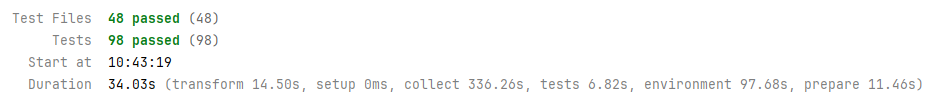
\includegraphics[width=0.8\textwidth]{TestResult.png}
	\caption{PetJoy项目测试结果}
\end{figure}

我们为项目中的每个组件和页面(即每个 Vue 文件)都专门配置了对应的测试文件,总共创建了48个测试文件,涵盖了98个单元测试。这些测试在开发过程中发挥了至关重要的作用,不仅确保了代码的质量,还显著提高了系统的稳定性,使我们能够快速发现和修复潜在问题,保证代码在各个功能模块中的可靠性。

